
В ходе проведения компьютерной экспертизы может возникнуть необходимость проанализировать электронные письма злоумышлиника, его контакты и прикрепленные  
файлы. Подобную информацию можно получить из файлов, сохраняемых программой OutLook  на ПК пользователя. Для  
осуществления данной задачи был разработан программный модуль Outlook 2007.

\subsubsection{Некоторые сведения о почтовых клиентах}

Почтовая программа (почтовый клиент, клиент электронной почты, мейлер, мейл-клиент) --- 
это ПО, которое инсталлируется на компьютер пользователя и предназначено для написания, получения, хранения, отправки электронной почты одного  
или нескольких пользователей (например, когда имеется несколько учетных записей на компьютере), или нескольких учетных записей пользователя. 


В  самом начале работы была найдена статья с расположением файлов сообщений, адресной книги, название прикрепленных файлов. В ходе поиска в  
операционной системе был найден только файл данных  pst, при разборе выяснилось, что данное расположение соответствует версии Outlook 2003, но она  
используется крайне редко, поэтому выбор пал на следующие версии  (Outlook 2007, Outlook 2010 и Outlook 2013), которые все данные хранят в бинарном  
файле pst. Версию  Outlook 2013 можно установить  в ОС Windows версии не ниже 7. Окончательно для дальнейшего написания программного модуля была выбрана версия Outlook 2007, так как на данную версию почтового клиента у разработчика имелась лицензия. 

\subsubsection{Реализация программного модуля}

Реализация данного программного модуля включала в себя следующие шаги:

\begin{enumerate}
\item Изучение проекта coex;
\item Изучение особенностей работы с библиотеками QT;
\item Изучение особенностей работы с XML-форматом (языка разметки);
\item Изучение системы компьютерной верстки  Latex для написания документации;
\item Изучение системы распределенного контроля версий Git и ее основных возможностей; 
\item Исследование почтового клиента Outlok 2007 (хранение логов и настроек);
\item Изучение различных файловых форматов, таких как PST, PAB, MSG, RTF, HTML;
\item Разработка программного модуля для сбора информации из почтового клиента MS Outlook и ее записи в XML-файл.
\end{enumerate}

\subsubsection{Исследование файловых форматов}

После нахождения файла, где хранится информация о интересующих нас данных,  
возник вопрос как считать эти данные, так как формат pst предназначен для открытия только программой  Outlook и является бинарным файлом. Для  
решения задачи и подтверждения предположения о том,что данный файл содержит интересующую нас информацию, была найдена программа Readpst для чтения формата  pst под  
операционной средой Linux. Но исходный код  данной программы не был найден.После чего возникла необходимость поиска способов
чтения и любых других действий с данным форматом. 

%рисунок - pst
Пример чтения файла в формате pst представлен на рисунке~\ref{pst:pst}.

\begin{figure}[h!]
\center{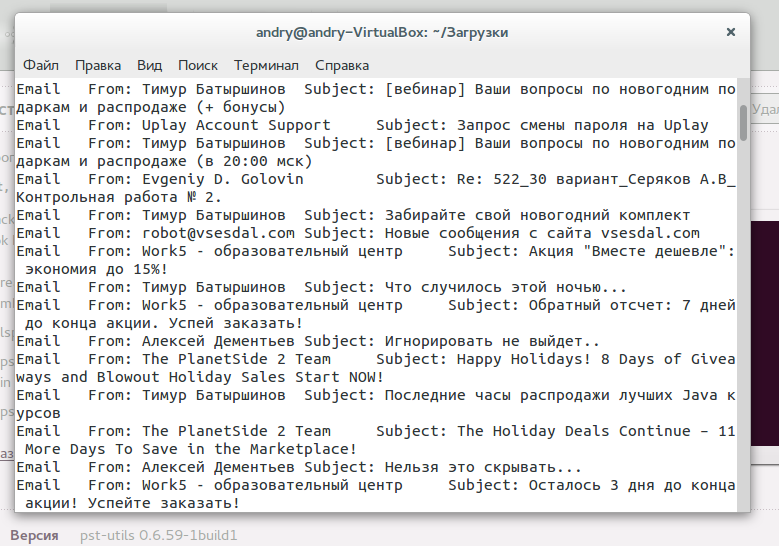
\includegraphics[width=0.6\linewidth]{pst}}
\caption{Чтение файла в формате pst}
\label{pst:pst}
\end{figure}

В статье от 2009 года компании Microsoft говорится о расшифровке и полном описании  
некоторых форматов MS. После прочтения данного документа был проведен поиск технического описания формата pst, в результате которого был найден архив с техническими описаниями некоторых форматов,в том  
числе и формата pst, на английском языке. В нем описана  основная структура. Файловые структуры Pst логически устраиваются в трех слоях, как это показано на рисунке~\ref{andrey_pic:andrey_pic}.

\begin{figure}[h!]                                                %рисунок - andrey_pic слои
\center{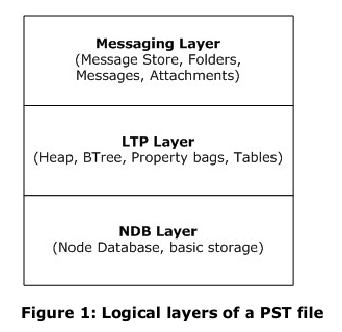
\includegraphics[width=0.6\linewidth]{andrey_pic}}
\caption{Cлой NDB}
\label{andrey_pic:andrey_pic}
\end{figure}

Слой NDB состоит из базы данных узлов, которая представляет склады низшего уровня 
формат файла PST. С точки зрения внедрения слой NDB состоит из заголовка, файла 
информации о распределении, блоков, узлов и двух BTrees: узел BTree (NBT) и блок BTree 
(BBT). NBT содержит ссылки на все доступные узлы в файле Pst. Его выполнение Btree 
позволяет в поиске размещать любой специфический узел. Bbt содержит ссылки на все  блоки данных файла Pst. Его выполнение Btree позволяет в поиске размещать любой специфический блок.


Слой Ltp (Списки, Таблицы, и Свойства) осуществляет высокоуровневые понятия сверху конструкции NDB. Основные элементы слоя LTP --- Property Context (PC) и Table Context (TC). PC представляет коллекцию 
свойства. TC представляет двумерный стол. Строки представляют коллекцию свойств. 
Колонки представляют свойства в пределах строк.


Передающий слой состоит из высокоуровневых правил и бизнес-логики, которые позволяют объединять структуры 
LTP и слои NDB и интерпретировать как объекты <<Папки>>, объекты <<Сообщения>>, 
объекты <<Приложения>> и <<Свойства>>. Передающий слой также определяет правила и требования.


Это сопровождается измением содержаниея файла PST так, чтобы измененный файл PST мог все еще быть успешно прочитан путем внедрения этого формата файла. 
Последовательности бит информации записываются в специальные  для них блоки,  что позволяет, опираясь на тег блока, брать нужное количество битовой информации для выборки интересующей нас информации.  Например: 0x1000001f -PidTagBody\_W-PtypBinary-58 Byte(s), 0x10130102-PidTagHtml-PtypBinary-1638 Byte(s), 0x1035001f-PidTagInternetMessageId\_W- PtypBinary-164 Byte(s), 0x3003001f -PidTagEmailAddress\_W-178 Byte(s). 


После чего был изучен код других плагинов для нахождения возможных  решений возникшей проблемы. В результате проведенных исследований были написаны два программных модуля, требущих дальнейшей модернизации. Первая программа ищет фалы разрешения pst и pab в папках стандратного размещения их в OutLook. Вторая программа считывает побитово файл pst и записывает полученные данные в строковую переменную.


Алгоритм поиска файлов в папках пользователей представлен на блок-схеме ниже (рис.~\ref{block_1_andrey:block_1_andrey} и~\ref{block_2_andrey:block_2_andrey}).

\begin{figure}[ht]                                                % 2 куска блок-схемы алгоритма
\center{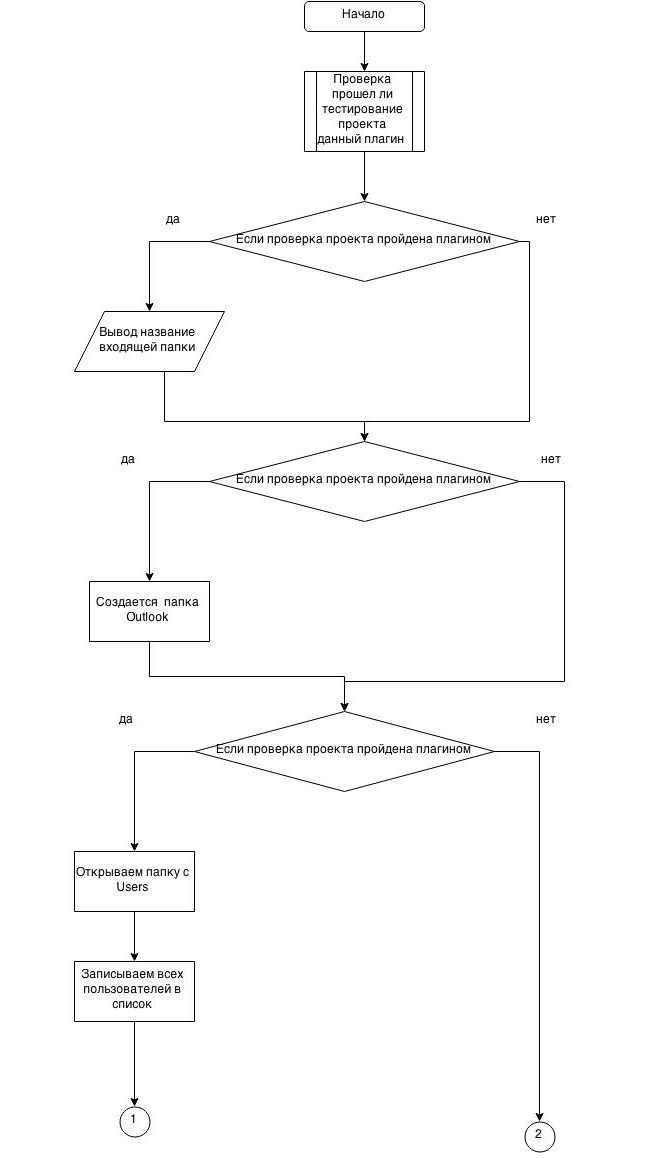
\includegraphics[width=0.6\linewidth]{block_1_andrey}}
\caption{Блок-схема алгоритма поиска файлов в папках пользователей}
\label{block_1_andrey:block_1_andrey}
\end{figure}

\begin{figure}[ht]
\center{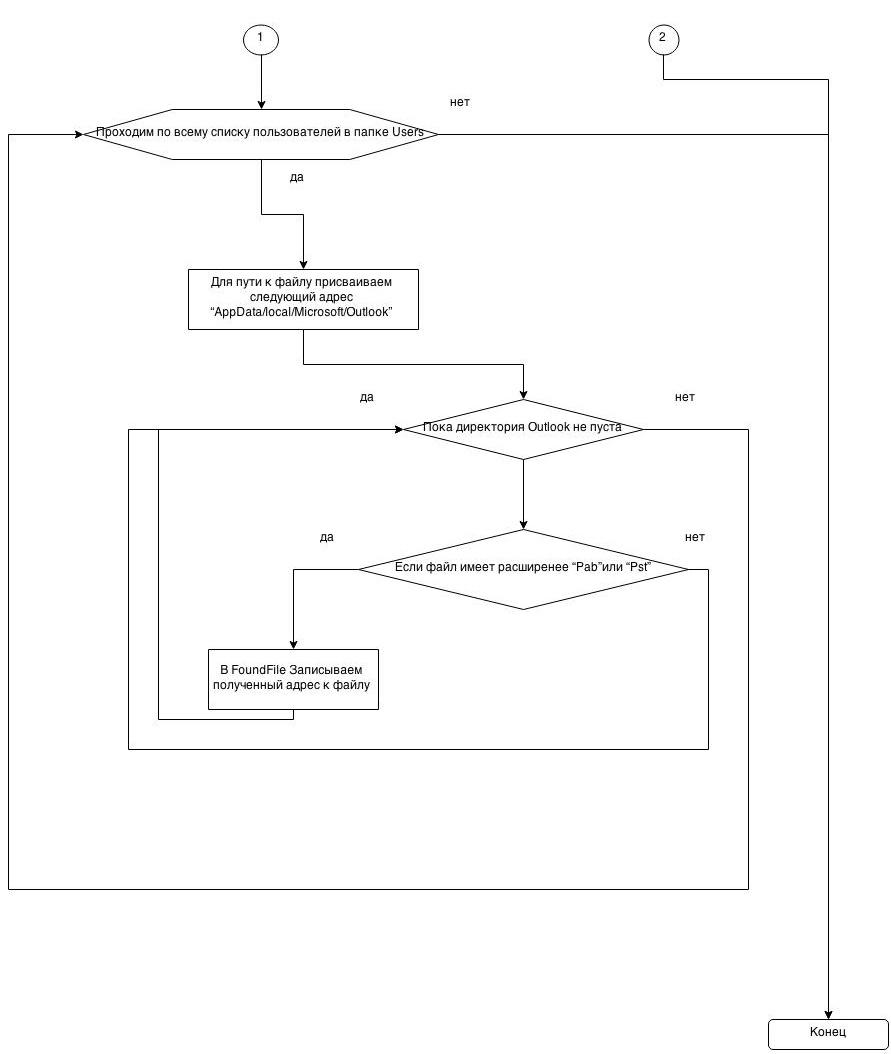
\includegraphics[scale=0.5]{block_2_andrey}}
\caption{Блок-схема алгоритма поиска файлов в папках пользователей (продолжение)}
\label{block_2_andrey:block_2_andrey}
\end{figure}

Побитовое считывание файла формата PST представлено на блок-схеме на рисунке~\ref{pst_reading:pst_reading}.

\begin{figure}[ht]                                                % блок-схема побитового чтения pst_reading
\center{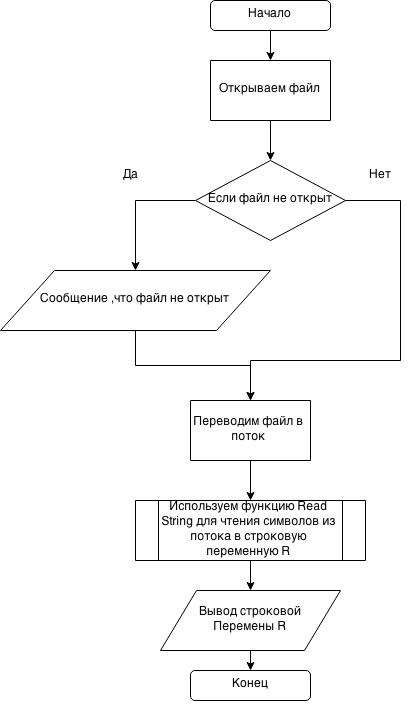
\includegraphics[width=0.6\linewidth]{pst_reading}}
\caption{Блок-схема алгоритма побитового считывания файла формата PST}
\label{pst_reading:pst_reading}
\end{figure}


\subsubsection{Задачи на следующий семестр}
В следующем семестре планируется переделать поиск фалов не только в стандартном расположении Outlook,но и в других директориях, за непродолжительное время. Также нужно модернизировать алгоритм чтения потока данных с фильтрацией ненужной информации, написать часть кода, в которой полученные данные будут записываться в xml-файл, изучить старые  возможные форматы хранения данных  pab, ost, msq, после чего написать функции работы с этими файлами в плагине Outlook2007 и записать  полученные данные в xml-файл. 

\clearpage
